\documentclass{article}

% if you need to pass options to natbib, use, e.g.:
%     \PassOptionsToPackage{numbers, compress}{natbib}
% before loading neurips_2024


% ready for submission
% \usepackage{neurips_2024}


% to compile a preprint version, e.g., for submission to arXiv, add add the
% [preprint] option:
     \usepackage[preprint]{neurips_2024}


% to compile a camera-ready version, add the [final] option, e.g.:
%     \usepackage[final]{neurips_2024}


% to avoid loading the natbib package, add option nonatbib:
%    \usepackage[nonatbib]{neurips_2024}


\usepackage[utf8]{inputenc} % allow utf-8 input
\usepackage[T1]{fontenc}    % use 8-bit T1 fonts
\usepackage{hyperref}       % hyperlinks
\usepackage{url}            % simple URL typesetting
\usepackage{booktabs}       % professional-quality tables
\usepackage{amsfonts}       % blackboard math symbols
\usepackage{nicefrac}       % compact symbols for 1/2, etc.
\usepackage{microtype}      % microtypography
\usepackage{xcolor}         % colors
\usepackage{amsmath}
\usepackage{natbib}
\usepackage{graphicx}  % For including graphics
\usepackage{float}     % To control figure placement
\usepackage{geometry}
\usepackage{array}
\usepackage{multirow}
\usepackage{graphicx}
\usepackage{subcaption}



\title{Deep Learning 1 - Homework 2}


% The \author macro works with any number of authors. There are two commands
% used to separate the names and addresses of multiple authors: \And and \AND.
%
% Using \And between authors leaves it to LaTeX to determine where to break the
% lines. Using \AND forces a line break at that point. So, if LaTeX puts 3 of 4
% authors names on the first line, and the last on the second line, try using
% \AND instead of \And before the third author name.


\author{%
  Pedro M.P.~Curvo \\
  MSc Artificial Intelligence\\
  University of Amsterdam\\
  \texttt{pedro.pombeiro.curvo@student.uva.nl} \\
  % examples of more authors
  % \And
  % Coauthor \\
  % Affiliation \\
  % Address \\
  % \texttt{email} \\
  % \AND
  % Coauthor \\
  % Affiliation \\
  % Address \\
  % \texttt{email} \\
  % \And
  % Coauthor \\
  % Affiliation \\
  % Address \\
  % \texttt{email} \\
  % \And
  % Coauthor \\
  % Affiliation \\
  % Address \\
  % \texttt{email} \\
}


\begin{document}


\maketitle


% \begin{abstract}
%   The abstract paragraph should be indented \nicefrac{1}{2}~inch (3~picas) on
%   both the left- and right-hand margins. Use 10~point type, with a vertical
%   spacing (leading) of 11~points.  The word \textbf{Abstract} must be centered,
%   bold, and in point size 12. Two line spaces precede the abstract. The abstract
%   must be limited to one paragraph.
% \end{abstract}


\section*{Part 1}

\subsection*{Question 1.1}

\subsubsection*{a)}

The expression for $f_{1, 1}$ is given by:

\begin{equation}
    f_{1, 1} = g_{1, 1} h_{0, 0} + g_{1, 2} h_{0, -} + g_{2, 1} h_{-, 0} + g_{2, 2} h_{-, -}
\end{equation}

As we can see, we didn't use the full receptive field of the filter, since it goes beyond the image.
To address this problem, we can pad the image using several techniques, such as zero-padding, reflection padding, warp padding, etc.

\subsubsection*{b)}

\subsubsection*{b. i)}

\begin{table}[h!]
    \centering
    \resizebox{\textwidth}{!}{%
    \setlength{\tabcolsep}{4pt}
    \renewcommand{\arraystretch}{1.2}
    \begin{tabular}{|c|c|c|c|c|c|c|c|c|c|c|c|c|c|c|}
    \hline
    \multirow{2}{*}{\textbf{Type}} & \multirow{2}{*}{\textbf{Dataset}} & \multicolumn{10}{c|}{Round Accuracy (\%)} & \multirow{2}{*}{\textbf{Mean}} & \multirow{2}{*}{\textbf{Std. Dev.}} \\ \cline{3-12}
                                   &                                  &  0 &  1 &  2 &  3 &  4 &  5 &  6 &  7 &  8 &  9 &  &  \\ \hline
    \multirow{2}{*}{Valid}     & Validation & 100.0 & 100.0 & 100.0 & 100.0 & 100.0 & 100.0 & 100.0 & 100.0 & 100.0 & 100.0 & 100.0000 & 0.0000 \\ \cline{2-14}
                               & Test       & 0.3   & 0.1   & 0.0   & 0.1   & 0.0   & 0.0   & 0.1   & 0.3   & 0.0   & 0.0   & 0.0900   & 0.1136 \\ \hline
    \multirow{2}{*}{Replicate} & Validation & 98.6  & 98.1  & 98.8  & 98.5  & 97.1  & 98.8  & 98.2  & 98.0  & 98.5  & 98.5  & 98.3100  & 0.4784 \\ \cline{2-14}
                               & Test       & 92.9  & 92.8  & 88.8  & 94.7  & 95.3  & 91.7  & 96.3  & 94.7  & 95.8  & 95.0  & 93.8000  & 2.1629 \\ \hline
    \multirow{2}{*}{Reflect}   & Validation & 100.0 & 100.0 & 100.0 & 100.0 & 100.0 & 100.0 & 100.0 & 100.0 & 100.0 & 100.0 & 100.0000 & 0.0000 \\ \cline{2-14}
                               & Test       & 0.0   & 0.0   & 0.0   & 0.0   & 0.0   & 0.0   & 0.0   & 0.0   & 0.0   & 0.0   & 0.0000   & 0.0000 \\ \hline
    \multirow{2}{*}{Circular}  & Validation & 99.9  & 99.9  & 99.7  & 99.9  & 98.9  & 99.7  & 99.7  & 99.5  & 99.8  & 99.4  & 99.6400  & 0.2939 \\ \cline{2-14}
                               & Test       & 81.5  & 82.7  & 77.4  & 86.9  & 83.2  & 82.6  & 86.5  & 79.8  & 81.1  & 84.4  & 82.6100  & 2.7504 \\ \hline
    \multirow{2}{*}{sconv}     & Validation & 98.8  & 99.0  & 98.8  & 99.1  & 99.0  & 99.3  & 98.7  & 98.8  & 98.9  & 98.5  & 98.8900  & 0.2119 \\ \cline{2-14}
                               & Test       & 6.5   & 6.9   & 6.5   & 6.1   & 6.2   & 6.5   & 6.2   & 6.1   & 6.4   & 6.3   & 6.3700   & 0.2326 \\ \hline
    \multirow{2}{*}{fconv}     & Validation & 88.4  & 87.6  & 88.6  & 89.9  & 88.1  & 89.9  & 85.8  & 87.1  & 88.2  & 87.1  & 88.0700  & 1.1984 \\ \cline{2-14}
                               & Test       & 88.4  & 88.6  & 88.6  & 89.9  & 89.1  & 89.9  & 88.9  & 88.4  & 88.9  & 87.8  & 88.8500  & 0.6249 \\ \hline
    \end{tabular}
    }
    \caption{Accuracy results for Net1}
    \label{tab:results_accuracy}
\end{table}

\subsubsection*{b. ii)}
Looking at the samples from the dataset, the pattern for class label 0 is to have a green on the right and a red on the left.
While the pattern for class label 1 is to have a red on the right and a green on the left.

The samples in the train set and the ones in the test set differ in the position of the green and red boxes, but
keeping the same pattern for each class label. For example, in the README.md, we can observe that the samples for
class label 0 are concentrated in the top ot the image and the samples for class label 1 are concentrated in the bottom
and in the test set, the samples for class label 0 are concentrated in the bottom and the samples for class label 1 are
concentrated in the top.
This means that the network will have to learn the pattern for each class label, regardless of the position of the boxes, 
i.e., the network will have to learn the pattern of the boxes and not the position of the boxes.

\subsubsection*{c)}

\subsubsection*{c i)}


The variables affecting the \texttt{conv\_type} are the \texttt{padding\_size} and the \texttt{pad\_type}.
For \textit{valid}, \textit{sconv} and \textit{fconv} we have the following differences:

\begin{itemize}
    \item \textit{valid}: No padding is added to the image, since the size of the padding is 0
    \item \textit{sconv}: The padding added is a zero padding, with size 1
    \item \textit{fconv}: The padding added is a zero padding, with size 2
\end{itemize}

\subsubsection*{c ii)}

If we look into the network architecture we can see that we first use a kernel size of 3 with a stride of 1 and then a stride of 2
maintaining the kernel size of 3. With this setup, the convolution operation will reduce the spatial dimensions
of the feature maps. 
By using the \textit{valid}, we are adding no padding to the image, which means that the output size of the convolution operation
will be the smallest of the tree. This lead to the reduction of the spatial dimensions of the feature maps, leading
to less spatial information being passed to the next layer.
\textit{sconv} retains slighty more spatial information, since we are adding a padding of 1 to the image, which will
lead to a slight increase in the output size of the convolution operation. This will lead to a slight increase in the spatial
information passed to the next layer.
\textit{fconv} retains the most spatial information, since we are adding a padding of 2 to the image, which will
lead to a significant increase in the output size of the convolution operation. This will lead to a significant increase in the spatial
information passed to the next layer.

With that being said, we can extrapolate that larger feature maps will keep more information that allows to distinguish
between the classes in the dataset, which leads to the better performance of the model in the accuracy metric as observed. 
Hence, the order \texttt{acc\_valid} $<$ \texttt{acc\_sconv} $<$ \texttt{acc\_fconv} is expected, corresponding
to the amount of spatial information retained by the feature maps.

\subsubsection*{c iii)}

The \texttt{reflect} padding mirrors the image along its edges, while \texttt{fconv} uses zero padding.
Reflect padding can reduce abrupt transitions at the edges by reflecting nearby pixel values,
but it can introduce patterns at the boundaries that do not exist in the original image.
These patterns can alter the feature extraction near the edges and might reduce the ability for the model to generalize.

In this dataset, where each image has a black background with one green box and one red box, zero padding performs better
as it adds zero-value borders that match the original black background,
allowing the network to focus on the actual box patterns.
Reflect padding, applied at all layers, can create artificial features at the edges, such as duplicating and inverting the boxes,
which may harm the model's ability to learn the actual patterns, since it can mix the patterns of the boxes.

\subsubsection*{c iv)}

Zero padding creates a sudden change in pixel values at the image boundaries, resulting in high derivative values across
the receptive fields near the edges. This can cause the CNN to confuse these abrupt changes with actual edges,
particularly the edges of the green and red boxes in the dataset that we are trying to predict.
The network may then interpret the zero padding as an actual feature, leading to worse performance in
edge detection, hence worse performance in identifying the boxes.

Replicate padding, on the other hand, extends the edge pixels into the padded area, ensuring a smoother transition, since
the pixel will have the same value as the nearest edge pixel. This helps preserve the local context near the edges by maintaining
some statistical properties of the image, such as the derivatives. This is beneficial
when detecting the edges of the boxes, since replicate padding prevents the network from confusing the padded area with the actual
edges. As a result, the replicate padding improves the model's performance in detecting the true edges of the boxes, leading
to a better accuracy.



\subsubsection*{d)}

\subsubsection*{d i)}
\begin{table}[h!]
    \centering
    \resizebox{\textwidth}{!}{%
    \setlength{\tabcolsep}{4pt}
    \renewcommand{\arraystretch}{1.2}
    \begin{tabular}{|c|c|c|c|c|c|c|c|c|c|c|c|c|c|c|}
    \hline
    \multirow{2}{*}{\textbf{Type}} & \multirow{2}{*}{\textbf{Dataset}} & \multicolumn{10}{c|}{Round Accuracy (\%)} & \multirow{2}{*}{\textbf{Mean}} & \multirow{2}{*}{\textbf{Std. Dev.}} \\ \cline{3-12}
                                   &                                  &  0 &  1 &  2 &  3 &  4 &  5 &  6 &  7 &  8 &  9 &  &  \\ \hline
    \multirow{2}{*}{Valid}     & Validation & 100.0 & 100.0 & 100.0 & 100.0 & 100.0 & 100.0 & 100.0 & 100.0 & 100.0 & 100.0 & 100.0000 & 0.0000 \\ \cline{2-14}
                               & Test       & 0.0   & 0.0   & 0.0   & 0.0   & 0.0   & 0.0   & 0.0   & 0.0   & 0.0   & 0.0   & 0.0000   & 0.0000 \\ \hline
    \multirow{2}{*}{Replicate} & Validation & 100.0 & 100.0 & 100.0 & 100.0 & 100.0 & 100.0 & 100.0 & 100.0 & 100.0 & 100.0 & 100.0000 & 0.0000 \\ \cline{2-14}
                               & Test       & 0.0   & 0.0   & 0.0   & 0.0   & 0.0   & 0.0   & 0.0   & 0.0   & 0.0   & 0.0   & 0.0000   & 0.0000 \\ \hline
    \multirow{2}{*}{Reflect}   & Validation & 100.0 & 100.0 & 100.0 & 100.0 & 100.0 & 100.0 & 100.0 & 100.0 & 100.0 & 100.0 & 100.0000 & 0.0000 \\ \cline{2-14}
                               & Test       & 0.0   & 0.0   & 0.0   & 0.0   & 0.0   & 0.0   & 0.0   & 0.0   & 0.0   & 0.0   & 0.0000   & 0.0000 \\ \hline
    \multirow{2}{*}{Circular}  & Validation & 100.0 & 100.0 & 100.0 & 100.0 & 100.0 & 100.0 & 100.0 & 100.0 & 100.0 & 100.0 & 100.0000 & 0.0000 \\ \cline{2-14}
                               & Test       & 0.0   & 0.0   & 0.0   & 0.0   & 0.0   & 0.0   & 0.0   & 0.0   & 0.0   & 0.0   & 0.0000   & 0.0000 \\ \hline
    \multirow{2}{*}{sconv}     & Validation & 100.0 & 100.0 & 100.0 & 100.0 & 100.0 & 100.0 & 100.0 & 100.0 & 100.0 & 100.0 & 100.0000 & 0.0000 \\ \cline{2-14}
                               & Test       & 0.0   & 0.0   & 0.0   & 0.0   & 0.0   & 0.0   & 0.0   & 0.0   & 0.0   & 0.0   & 0.0000   & 0.0000 \\ \hline
    \multirow{2}{*}{fconv}     & Validation & 100.0 & 100.0 & 100.0 & 100.0 & 100.0 & 100.0 & 100.0 & 100.0 & 100.0 & 100.0 & 100.0000 & 0.0000 \\ \cline{2-14}
                               & Test       & 0.0   & 0.0   & 0.0   & 0.0   & 0.0   & 0.0   & 0.0   & 0.0   & 0.0   & 0.0   & 0.0000   & 0.0000 \\ \hline
    \end{tabular}
    }
    \caption{Accuracy results for Net2}
    \label{tab:results_accuracy_net2}
\end{table}

\subsubsection*{d ii)}

As we can observe by the results, the model is able to achieve 100\% accuracy on the validation set for all padding types, 
but it fails to generalize to the test set, achieving 0\% accuracy, performing worse in every padding type in \texttt{Net2}
with lower accuracies than \texttt{Net1}.

\subsubsection*{d iii)}

In the \texttt{Net2}, we added an additional linear layer and we remove the AdaptiveMaxPool2d layer. 
The additional linear layer increases exponentially the number of parameters in the model, which can lead to overfitting.
If we look into the \texttt{utils.py} file, we can see the the test dataset is shifted by 16 pixels relative to the validation
and training dataset. This can mean that the model \texttt{Net2} is overfitting to the training and validation dataset
by memorizing the overall positions of the boxes and, since they are shifted in the test dataset, the model is unable to
generalize to the test dataset, leading to the 0\% accuracy. This makes sense if we also consider that the model
is achieving 100\% accuracy in the validation set, while getting 0\% accuracy in the test set in all padding types.

\subsection*{Question 1.2}

\subsubsection*{a)}

% Include image the plot of inference respect to angle of rotation 
\begin{figure}[H]
    \centering
    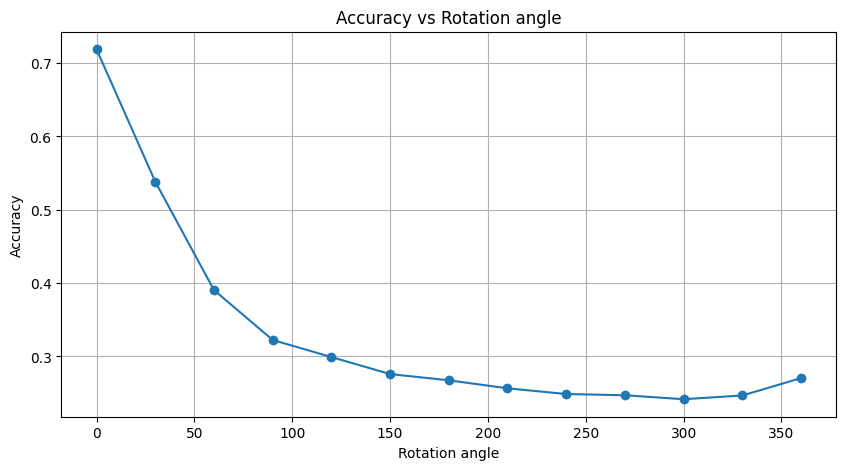
\includegraphics[width=0.8\textwidth]{images/rot_angles.png}
    \caption{Inference respect to angle of rotation}
    \label{fig:angle_inference}
\end{figure}

CNNs are not naturally rotationally invariant because the filters they learn during training are sensitive to the orientation
of features in the images. When an image is rotated, the learned filters may no longer align with the features in the new
orientation. This misalignment reduces the model's ability to recognize patterns, leading to a drop in accuracy. The
convolutional layers detect local patterns such as edges and textures in a fixed direction, and rotating the image changes
the spatial relationships between these features, making it harder for the network to match them correctly.

If the model is not trained on rotated images, it cannot learn to recognize objects or patterns from different angles.
The performance of the model is highly dependent on the orientation of the test images, and it is likely to perform worse
when presented with images that were not seen during training. Even though the model might perform better at certain rotation
angles (e.g., 90° or 180°), accuracy typically drops as the angle deviates from those orientations. This demonstrates that
CNNs require rotation-invariant training data or additional techniques like data augmentation to improve their ability to
recognize rotated images.

\subsubsection*{b)}

% Include image the plot of inference respect to angle of rotation
\begin{figure}[H]
    \centering
    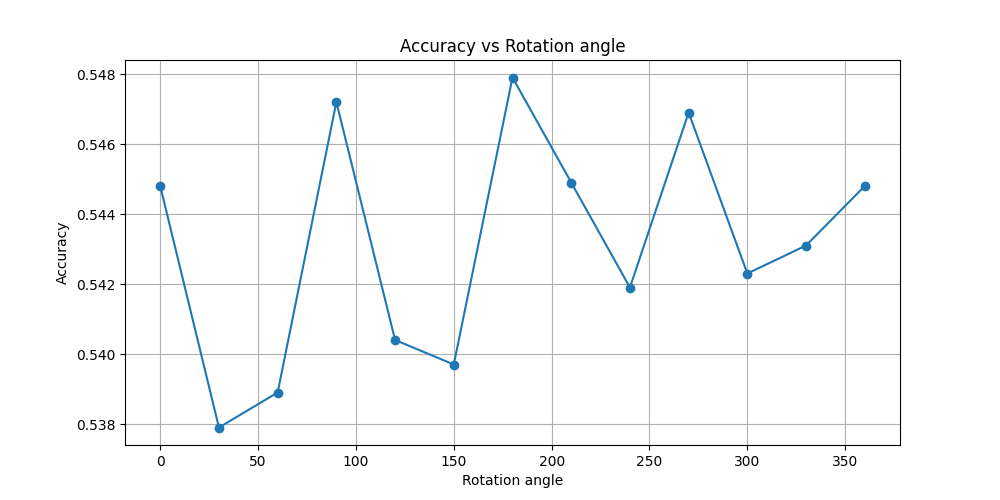
\includegraphics[width=0.8\textwidth]{images/rot_angles_aug.png}
    \caption{Inference respect to angle of rotation with data augmentation}
    \label{fig:angle_inference_aug}
\end{figure}

When the model is trained on an augmented dataset with random rotations, it is exposed to a wide variety of orientations for
the objects in the images. This allows the model to learn features that are not dependent on a specific orientation. By
incorporating rotated versions of the images during training, the model learns to recognize patterns and objects regardless
of their angle. This helps the network develop rotational invariance, as the filters it learns become capable of detecting
the same features from different perspectives.

As a result, the model becomes more robust to rotation, and its accuracy stabilizes across different angles during inference.
With this training approach, the network does not rely on a fixed alignment of the features, and can instead generalize across
a range of orientations. This improved performance across various rotation angles indicates that the network has learned to
identify the objects or patterns in the images without being influenced by their orientation, thereby overcoming the limitations
of rotational sensitivity found in networks trained only on images with fixed orientations.

\newpage

\section*{Part 2}

\subsection*{Question 2.1}

\subsubsection*{a)}

\begin{itemize}
    \item Long input sequences can be challenging for Transformers due to the quadratic complexity of the self-attention mechanism, 
    that is, in self-attention, each token attends to every other token in the sequence, hence we have a  
    $O(n^2)$ complexity that can be seen by multiplying the $Q$, $K$ and $V$ matrices. This can lead to both memory
    and computational issues, which are worse when $n$ is large (larger sentences).

    \item One way to solve this problem is by using some kind of sparse attention mechanism that focus on a subset
of local or key tokens. With this we can reduce the complexity of the self-attention mechanism. For example,
the Reformer model~ %\cite{Kitaev2020}%
 uses locality-sensitive hashing to achieve a $O(n \log n)$ complexity.
\end{itemize}

\subsubsection*{b)}

CNNs have a local receptive field that allows them to capture local patterns in the input data and which is done
by the convolution operation between the input and a kernel filter. One the other hand, Transformers have a global
receptive field that allows them to capture long-range dependencies in the input data, which is done by the self-attention
mechanism, since it allows each token to attend to every other token in the sequence.

\subsubsection*{c)}

The scaling factor $\frac{1}{\sqrt{d_k}}$ is used to stabilize the gradients during training. The dot product of the
$Q$ and $K$ matrices is scaled by $\frac{1}{\sqrt{d_k}}$ to prevent the dot products from becoming too large when the
dimensionality of the keys $d_k$ is high. If it were the case that some values were too large, the softmax function would
produce gradients that are too small, leading to slower learning or vanishing gradients which would harm the gradient descent process.

\subsubsection*{d)}

If we assume we have the same total computation cost then the multiple attentions heads are beneficial because they allow
to capture different types of dependencies and patterns simultaneously. Each attention head can focus on different parts of the
input sequence, like in CNNs we have several filters. It can also help mitigate some bias that can originate in some
heads due to the dominance of some tokens and can help improve generalization because, by learning multiple sets of
attention parameters, the model can be more robust to different tasks.


\subsection*{Question 2.2}

\textcolor{blue}{CODE}

\subsection*{Question 2.3}

\subsubsection*{a to b)}
\textcolor{blue}{CODE}

\subsubsection*{c)}

The MLP head is wide and not deep for several factors.
In one hand, we want to keep independence of tokens in the MLP, meaning we don't need a deep network to capture
the dependencies between the tokens. With a wide network, we are basically representing each token in a higher-dimensional
space, which can help to capture more complex patterns independently. If we employed a deep network, we would be
capturing dependencies between tokens, which is not necessary in this case, since the self-attention mechanism already
does it.
In the other hand, with a wide network we can apply a parallel computation, that is, splitting the model across multiple
GPUs, which can lead to more computational efficiency. By keeping the MLP shallow, we also reduce the probability of overfitting
and can keep a more stable training process.


\subsection*{Question 2.4}

\subsubsection*{a)}

If we do not use a positional embedding, the Transformer model will not be able to distinguish the order of the tokens in the
input sequence. This is because the self-attention mechanism treats all tokens as independent, and without positional information,
meaning is permutation invariant. For example, without positional embeddings, the model would treat the sentences "The dog bit the man"
and "The man bit the dog" as the same, which is not the desired behavior. We need to have a positional embedding
for a sequential structure, specially for tasks like syntax, etc... which are characteristics of LLMs.

\subsubsection*{b)}

By using absolute position embeddings, that is, by assigning, for example, 1 to the first token, 2 to the second token, and so on,
we are restricting the model to work within the predefined sequence length. This can be problematic if we then want to apply the model
to sequences that are longer than the ones seen during training. Besides that, we can have, for example, different types of inputs, 
where lengths can vary, for example, documents, translation tasks, etc... In these cases, the model would not be able to generalize.
Adding to this, we also want the model to have a sense of proximity between tokens, which is not achieved by absolute position embeddings.
For example, we might want the model to understand that the tokes "The" and "dog" appear closer than "man" and "dog".

By using relative position embeddings, we can overcome these limitations. Relative position embeddings allow the model to learn
the relative distances between tokens, which can be more useful in tasks where the absolute position of tokens is not as important.
Adding to this, the model can then extrapolate to different new sequences lengths and can even retain the context in large
sequences, for example, in resuming tasks, where we have large documents.


\subsection*{Question 2.5}

\textcolor{blue}{CODE}

\subsection*{Question 2.6}

\textcolor{blue}{CODE}

\subsection*{Question 2.7}

% Insert image with epochs
\begin{figure}[H]
    \centering
    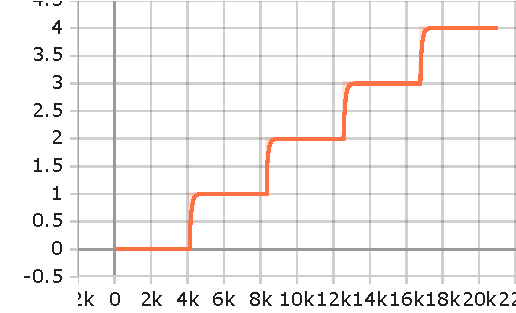
\includegraphics[width=0.8\textwidth]{images/epoch.pdf}
    \caption{Epochs per Step}
    \label{fig:loss_epochs}
\end{figure}

% Insert image with Train Acc Epoch 

\begin{figure}[H]
    \centering
    \begin{subfigure}{0.48\textwidth}  % Adjust the width to your preference
        \centering
        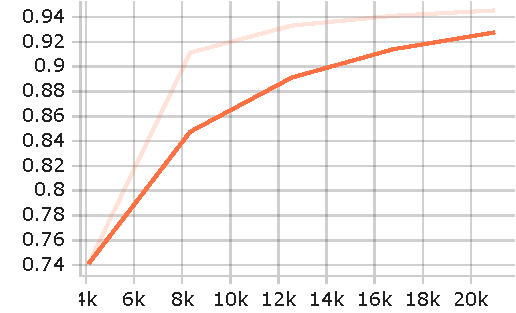
\includegraphics[width=\textwidth]{images/train_acc_epoch.pdf}
        \caption{Train Accuracy per Epoch}
        \label{fig:train_acc_epochs}
    \end{subfigure}
    \hfill
    \begin{subfigure}{0.48\textwidth}
        \centering
        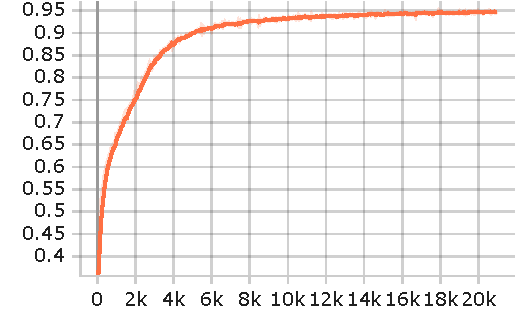
\includegraphics[width=\textwidth]{images/train_acc_step.pdf}
        \caption{Train Accuracy per Step}
        \label{fig:train_acc_steps}
    \end{subfigure}
\end{figure}

% Insert image with Train Loss per Epoch

\begin{figure}[H]
    \centering
    \begin{subfigure}{0.48\textwidth}  % Adjust the width to your preference
        \centering
        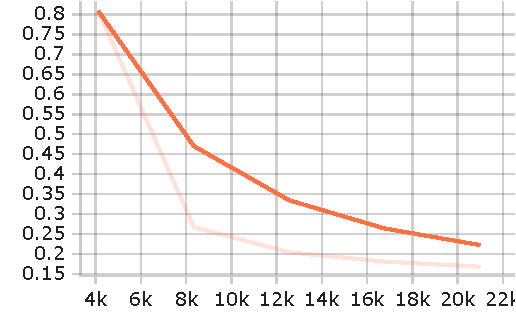
\includegraphics[width=\textwidth]{images/train_loss_epoch.pdf}
        \caption{Train Loss per Epoch}
        \label{fig:train_loss_epochs}
    \end{subfigure}
    \hfill
    \begin{subfigure}{0.48\textwidth}
        \centering
        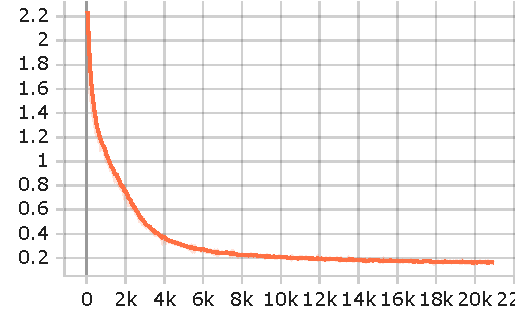
\includegraphics[width=\textwidth]{images/train_loss_step.pdf}
        \caption{Train Loss per Step}
        \label{fig:train_loss_steps}
    \end{subfigure}
\end{figure}

\subsection*{Question 2.8}

\subsubsection*{a)}

\textcolor{blue}{CODE}
\textcolor{red}{TODO: REVISE}

\subsubsection*{b)}

\textcolor{red}{TODO: just need to put some prompts here}

\subsection*{Question 2.9}

\subsubsection*{a)}

\textcolor{blue}{CODE}
\textcolor{red}{TODO: REVISE}

\subsubsection*{b)}

\newpage

\section*{Part 3}

\subsection*{Question 3.1}

\subsubsection*{a)}

For the first graph we have:

$[
[0, 1, 1, 0, 1],
[1, 0, 1, 0, 0],
[1, 1, 0, 1, 0],
[0, 0, 1, 0, 0],
[1, 0, 0, 0, 0]]$

For the second graph we have:

$[
[0, 1, 0, 0, 0, 0],
[1, 0, 1, 0, 1, 0],
[0, 0, 1, 0, 1, 0],
[0, 0, 1, 0, 1, 1],
[0, 1, 0, 1, 0, 1], 
[0, 0, 0, 1, 1, 0]]$

\subsubsection*{b)}

By squaring the first adjacency matrix we have:

$[
[3, 1, 1, 1, 0],
[1, 2, 1, 1, 1],
[1, 1, 3, 0, 1],
[1, 1, 0, 1, 0],
[0, 1, 1, 0, 1]]$

When we square the matrix $A \rightarrow A^2$, we are counting the number of paths of length 2 between each pair of nodes,
that is, $A_{ij}^2$ is the number of paths of length 2 between nodes $i$ and $j$.
For example the entry $A_{12}^2 = 1$ means that there is 1 path of length 2 between nodes 1 and 2, which is the path
$1 \rightarrow 3 \rightarrow 2$.

More generally, the entry $A_{uv}^n$ is the sum of the number of paths of length $n$ between nodes $u$ and $v$ in the graph.

\textbf{Note:} In the diagonals we have the number of paths of length 2 that start and end in the same node, for example,
if node $1$ and $5$ are connected this represents also a path of length 2, because we can go from node $1$ to node $5$ and
then back to node $1$. This is only true in the case of undirected graphs.

\subsubsection*{c)}

The Laplacian matrix is defined as $L = D - A$, where $D$ is the degree matrix and $A$ is the adjacency matrix.
The degree matrix is a diagonal matrix where the diagonal entries are the sum of the weights of the edges connected to each node.

For the second graph we have that $D$ is:

$[
[1, 0, 0, 0, 0, 0],
[0, 3, 0, 0, 0, 0],
[0, 0, 2, 0, 0, 0],
[0, 0, 0, 3, 0, 0],
[0, 0, 0, 0, 3, 0],
[0, 0, 0, 0, 0, 2]]$

And the Laplacian matrix is:

$[
[1, -1,  0, 0, 0, 0],
[-1, 3, -1, 0, -1, 0],
[0, -1,  2, 0, -1, 0],
[0, 0,  -1, 3, -1, -1],
[0, -1,  0, -1, 3, -1],
[0, 0,   0, -1, -1, 2]]$

By applying the Laplacian matrix to an input matrix $X$, we have that $F = L \cdot X$. 
If we consider the way matrix multiplication works, we see that $F$ is the result of the span of the row space of $X$ by the columns of $L$.
The columns of $L$ have larger value if $D$ is larger, that is, if the node is more connected to other nodes, which means that
if a node has high degree, it will be more influenced by its neighbors because the corresponding row in $L$ will have larger values.
We can conclude, in this case, that the nodes that change the most are nodes $2$, $4$ and $5$, since they have higher degree $(3)$.

\textcolor{red}{NEEDS REVISION}





























\newpage
\bibliographystyle{abbrvnat}
\bibliography{references} 


\end{document}